% arara: xelatex
% arara: xelatex
% arara: xelatex


% options:
% thesis=B bachelor's thesis
% thesis=M master's thesis
% czech thesis in Czech language
% english thesis in English language
% hidelinks remove colour boxes around hyperlinks

\documentclass[thesis=M,english]{FITthesis}[2012/10/20]

\usepackage[utf8]{inputenc} % LaTeX source encoded as UTF-8
% \usepackage[latin2]{inputenc} % LaTeX source encoded as ISO-8859-2
% \usepackage[cp1250]{inputenc} % LaTeX source encoded as Windows-1250

\usepackage{graphicx} %graphics files inclusion
% \usepackage{subfig} %subfigures
\usepackage{amsmath} %advanced maths
\usepackage{amssymb} %additional math symbols

\usepackage{dirtree} %directory tree visualisation
\usepackage{relsize}

\usepackage{amsthm} 
\theoremstyle{remark}
\newtheorem*{RM}{Remark}

\newtheorem*{NRM}{Notational Remark}

\theoremstyle{definition}
\newtheorem{DF}{Definition}[section]

% % list of acronyms
% \usepackage[acronym,nonumberlist,toc,numberedsection=autolabel]{glossaries}
% \iflanguage{czech}{\renewcommand*{\acronymname}{Seznam pou{\v z}it{\' y}ch zkratek}}{}
% \makeglossaries

% % % % % % % % % % % % % % % % % % % % % % % % % % % % % % 
% EDIT THIS
% % % % % % % % % % % % % % % % % % % % % % % % % % % % % % 

\department{Department of Information Security}
\title{Summation polynomials and the discrete logarithm problem on elliptic curve}
\authorGN{Matyáš} %author's given name/names
\authorFN{Hollmann} %author's surname
\author{Matyáš Hollmann} %author's name without academic degrees
\authorWithDegrees{Bc. Matyáš Hollmann} %author's name with academic degrees
\supervisor{Ing. Ivo Petr, Ph.D.}
\acknowledgements{THANKS (remove entirely in case you do not with to thank anyone)}
\abstractEN{Summarize the contents and contribution of your work in a few sentences in English language.}
\abstractCS{V n{\v e}kolika v{\v e}t{\' a}ch shr{\v n}te obsah a p{\v r}{\' i}nos t{\' e}to pr{\' a}ce v {\v c}esk{\' e}m jazyce.}
\placeForDeclarationOfAuthenticity{Prague}
\keywordsCS{Replace with comma-separated list of keywords in Czech.}
\keywordsEN{Replace with comma-separated list of keywords in English.}
\declarationOfAuthenticityOption{4} %select as appropriate, according to the desired license (integer 1-6)
% \website{http://site.example/thesis} %optional thesis URL


\begin{document}

% \newacronym{CVUT}{{\v C}VUT}{{\v C}esk{\' e} vysok{\' e} u{\v c}en{\' i} technick{\' e} v Praze}
% \newacronym{FIT}{FIT}{Fakulta informa{\v c}n{\' i}ch technologi{\' i}}

\setsecnumdepth{part}
\chapter{Introduction}

\setsecnumdepth{all}
\chapter{Mathematical Background}\label{mathBG}
%\input{mathBG.tex}
 %definice pojmu, finite fields, etc.
 In this chapter we are going to define terms that will be used in the rest of this thesis. The first section is a revision of terms common in general algebra, the second section is focused on polynomials and Gröbner bases and the last section will deal with elliptic curves. This chapter is based mostly on book by David A. Cox \cite{algGeom}, MI-MKY lecture notes \cite{mky} and my bachelor thesis \cite{myBP}. Other sources will be cited individually at the specific locations.
\section{Introduction to General Algebra}
General algebra, also called universal algebra in the past, is the theory of algebraic structures. An algebraic structure is a set of objects with a collection of mathematical operations on this set.  An algebraic structure is defined by a set of axioms, requirements on the set and operations on it, and logically deduce other properties of said algebraic structure based on the axioms. When we encounter a particular problem we may try to classify it as a specific algebraic structure (by verifying its axioms) and use all of its deduced properties without the need to reprove them. We start this section with a definition of an elementary algebraic structure called group.
\begin{DF}
A \textbf{group} $G$ is an ordered pair $(M,  \circ)$, where $M$ is a non-empty set and binary operation $\circ : M \times M \to M $ (sometimes called the group law of $G$) that satisfies three requirements known as group axioms: 
\end{DF}
\begin{itemize}
\item 
$ \forall x,y,z \in M: x\circ (y \circ z) = (x \circ y) \circ z,$ \hfill (associativity)
\item 
$ \exists e \in M,\ \forall x \in M: e \circ x = x \circ e = x,$ \hfill (identity element)
\item 
$\forall x \in M,\ \exists x^{-1} \in M: x \circ x^{-1} = x^{-1} \circ x = e.$ \hfill (inverse element)
\end{itemize}
\begin{RM}
$M$ is closed under the operation $\circ$. 
\end{RM}
\begin{NRM}
When we are gonna talk about an element  $g$ of a group $G$ ($g \in G$) we are actually gonna mean that $g$ is an element of the underlying set $M$ ($g \in M$).
\end{NRM}
Groups satisfying commutativity law:
\begin{itemize}
\item 
$ \forall x, y\in M: x \circ y = y \circ x,$
\end{itemize}
are called \textbf{Abelian groups} (in honour of a famous Norwegian mathematician Niels Henrik Abel). 
\begin{DF}
If the set $M$ has a finite number of elements, $G = (M, \circ)$ is called a \textbf{finite group}. \textbf{Order} of the finite group $G$ is the number of elements of the underlying set $M$ and we denote it by $\#G$. If the set $M$ is infinite, the order of $G$ is infinite as well.
\end{DF}
\noindent A simple example of an infinite Abelian group is $(\mathbb{Z}, +)$, set of all integers equipped with standard addition. An example of a finite Abelian group is $\mathbb{Z}_n^+ = (\{0, 1, \ldots, n-1\}, +_{n}),\ n \in \mathbb{N},$ where $+_n$ is addition modulo $n$ and $\mathbb{N}$ is the set of all natural numbers (positive integers). Order of this group is $n$.
\begin{RM}
In every group there exist just one unique identity element. Also for every element $q \in G$ there exists just one inverse element denoted $q^{-1}$ in the multiplicative notation and $-q$ in the additive notation. Inverse of a product of two group elements is a product of the respective inverses in the reversed order (order does matter in non-commutative groups), although in this thesis we are mostly concerned about commutative groups.
\end{RM}
\noindent Identity element in the additive notation is called \textbf{zero} and denoted by $0$, in the multiplicative notation \textbf{unit} and denoted by $1$. \\ \\
In an additive group $G$ we define \textbf{multiplication} by an integer (repeated application of the group law) as follows:
$$
\forall p \in G,\ \forall k \in \mathbb{Z}: kp := \begin{cases} \underbrace{p + p + \cdots + p}_{\text{k-times}} &\quad k > 0, \\
0 \text{ (identity element) } &\quad k = 0, \\
\underbrace{(-p) + (-p) + \cdots + (-p)}_{\text{k-times}} &\quad k < 0.
\end{cases}
$$
In a multiplicative group $G$ we define \textbf{exponentiation} (repeated application of the group law) in a similar manner:
$$
\forall p \in G,\ \forall k \in \mathbb{Z}: p^k := \begin{cases} \underbrace{p \cdot p \cdots  p}_{\text{k-times}} &\quad k > 0, \\
1 \text{ (identity element) } &\quad k = 0, \\
\underbrace{p^{-1} \cdot p^{-1} \cdots  p^{-1}}_{\text{k-times}} &\quad k < 0.
\end{cases}
$$
\begin{DF}
\textbf{Order of an element} $a \in G$ is the smallest positive integer $k \in \mathbb{N}$ such that: $a^k = 1$ (similarly $ka = 0$ in the additive notation), we denote it by $\#a= k$, if there isn't such $k$, we say the order of $a$ is infinite (this case may only happen if $G$ itself is of infinite order and in this thesis we are mostly interested in finite groups). Elements of finite order are sometimes called \textbf{torsion} elements.
\end{DF}
\begin{RM}
Order of the identity element $\in G$ is always $1$ and due to the uniqueness of the identity element it's also the only element $\in G$ of this order.
\end{RM}
\begin{DF}
A group $(H, \circ)$ is a \textbf{subgroup} of a group $(G, \circ)$ if and only if $H \subseteq G.$ The group law $\circ$ is exactly the same, therefore the identity element $e \in G$ has to be the identity in any subgroup $H$ of $G$ as well. $H$ is called a \textbf{trivial subgroup} of $G$ if $H = \{e\}$ or $H = G$.
\end{DF}
\begin{DF}
\textbf{Lagrange's Theorem}: Let $G$ be a finite group and $H$ a subgroup of $G$, then the order of the subgroup $H$ divides the order of the group $G$: $\exists n \in \mathbb{N}: \#G = \#H \cdot n.$
\label{lagrange}
\end{DF}
\begin{DF}
A \textbf{relation} $\mathcal{R}$ on a set $M$ is any subset of the Cartesian product $M\times M$. Relation $\mathcal{R}$ on the set $M$ is an \textbf{equivalence} on the set $M$ if and only if $\mathcal{R}$ satisfies following requirements:
\begin{itemize}
\item $\forall	x \in M: (x,x) \in \mathcal{R},$ \hfill (reflexivity)
\item $\forall x,y \in M: (x,y) \in \mathcal{R} \implies (y,x) \in \mathcal{R},$ \hfill (symmetry)
\item $\forall x,y,z \in M: \bigg( (x,y) \in \mathcal{R} \land (y,z) \in \mathcal{R}\bigg) \implies (x,z) \in \mathcal{R}.$ \hfill (transitivity)
\end{itemize}
\end{DF}
\noindent Set of all elements equivalent to $x \in M$ is called an \textbf{equivalence class} of an element $x$ and denoted by:
$$
[x]_\mathcal{R} := \{y \in M \ |\ (x,y) \in \mathcal{R}\}.
$$
\begin{NRM}
Let $\mathcal{R}$ be an equivalence relation on a set $M$, to denote the equivalence of $x,y \in M$ we will shorten the notation to $x \sim_\mathcal{R} y := (x,y) \in \mathcal{R}.$ 
\end{NRM}
\noindent For any subgroup $H$ of a group $G$ and an element $a \in G$, we define a \textbf{left coset} of $H$ as $aH := \{ah\ |\ h \in H\}$. Similarly a \textbf{right coset} of $H$ is defined as $Ha := \{ha\ |\ h \in H\}$.  We also define an equivalence relation $\sim_{\mathcal{H}}$ by: 
$$
x,y \in G: (x \sim_{\mathcal{H}} y) \Leftrightarrow (\exists h \in H: x = yh).
$$
The equivalence classes ($[a]_{\mathcal{H}} = \{ah\ |\ h \in H \}$) of the equivalence relation $\sim_{\mathcal{H}}$ are exactly the left cosets of $H$ so we can write $[a]_{\mathcal{H}} = aH$. Thus the left cosets of $H$ form a partition of $G$, see \cite{coset}.
\begin{RM}
If $G$ is an Abelian group and $H$ is any subgroup of $G$, the left cosets of $H$ are the same as the right cosets of $H$, $H$ is then called \textbf{normal subgroup} of $G$. 
$$
\forall a \in G: aH = Ha.
$$ 
\end{RM} 
\noindent In the case $H$ is a normal subgroup of $G$ we can extend the group law ($\circ$) of $G$ to the the set of (left) cosets of $H$ as follows:
$$
\forall a,b \in G: [a]_{\mathcal{H}} \circ [b]_{\mathcal{H}} := [a \circ b]_{\mathcal{H}}.
$$
\begin{DF}
The ordered pair $(\{[a]_{\mathcal{H}}\ |\ a \in G\}, \circ)$ forms a \textbf{factor group} (sometimes called a \textbf{quotient group}) of $G$ with respect to $H$ and we denote it by $G/H$.
\end{DF}
\begin{DF}
Group $G$ is called a \textbf{cyclic group} if and only if there exists an element $g \in G$ such that:
\begin{itemize}
\item $G = \langle g \rangle := \{ g^n\ |\ n \in \mathbb{Z} \},$ \hfill (in the multiplicative notation) 
\end{itemize}
or
\begin{itemize}
\item $G = \langle g \rangle := \{ ng\ |\ n \in \mathbb{Z} \}.$ \hfill (in the additive notation)
\end{itemize}
\end{DF}
\noindent Element $g$ is then called a \textbf{generator} of the group $G$.
\begin{RM}
Ordered pair $(\langle a \rangle, \circ)$ form a subgroup of $(G, \circ)$ for any $a \in G$. Order of the group generated by the element $a$ is the same as order of the element~$a$. 
$$
\forall a \in G: \#\langle a \rangle = \#a.
$$
\end{RM}

\begin{DF}
An (unital) \textbf{ring} $R = (M, +, \cdot)$  is a set equipped with two binary operations $+: M\times M \to M$ and $\cdot:  M\times M \to M$ satisfying following requirements:
\begin{itemize}
\item $(M, +)$ is an Abelian group, 
\item $\forall x,y,z \in M: x\cdot(y\cdot z) = (x \cdot y) \cdot z, $ \hfill (associativity)
\item $\exists e \in M,\forall x \in M: e \cdot x = x \cdot e = x,$ \hfill (identity element w.r.t. operation $\cdot$)
\item $\forall x,y,z \in M:x \cdot(y+z)= x\cdot y + x \cdot z,$ \hfill (left distributive law) 
\item $\forall x,y, z \in M:(y + z) \cdot x = y\cdot x + z \cdot x.$ \hfill(right distributive law)
\end{itemize}
\end{DF}
\begin{NRM}
When we are gonna talk about an element $r$ of a ring $R$ ($r \in R$) we are actually gonna mean that $r$ is an element of the underlying set~$M$ ($r \in M$).
\end{NRM}
\begin{DF}
Let $R = (M,+,\cdot)$ be an unital ring and $(M \setminus \{0\}, \cdot)$ be an Abelian group, then $\mathbb{F} = (M, +, \cdot)$ is a \textbf{field}. Group $(M, +)$ is  called the additive group of the field $\mathbb{F}$ and denoted by $\mathbb{F}^+$, the identity element of this group is denoted by~$0$. Group $(M \setminus \{0\}, \cdot)$ is called the multiplicative group of the field $\mathbb{F}$ and denoted by $\mathbb{F}^\times$, the identity element of this group is denoted by~$1$.
\end{DF}
\begin{DF}
Let $\mathbb{F}$ be a field, 0 be the identity element of $\mathbb{F}^+$ and 1~be the identity element of $\mathbb{F}^\times$, if there exists such $n \in \mathbb{N}:$
$$
 \underbrace{1 + 1 + \cdots + 1}_\text{n-times} = 0,
$$ we define the smallest $n \in \mathbb{N}$ satisfying this condition to be the \textbf{characteristic} of the field $\mathbb{F}.$ If there isn't such $n$ we define the characteristic of the field $\mathbb{F}$ to be $0$. We denote the characteristic of the field $\mathbb{F}$ by char$(\mathbb{F})$.
\end{DF}
\noindent The characteristic of a field is either $0$ or a prime number. An example of a field of characteristic $0$ are real numbers with standard addition and multiplication $(\mathbb{R}, +, \cdot)$. \\ \\
An example of a field of prime characteristic $p$ is a set of non-negative integers less than $p$ equipped with addition modulo $p$ and multiplication modulo~$p$ $(\{0, 1, \ldots, p-1\}, +_p, \cdot_p)$, we call this field the \textbf{Galois Field} of order $p$ (order of a field is defined as the order of its additive group) and denote it by $GF(p)$.

\begin{RM}
All finite fields (fields with finite number of elements) are of prime characteristic. 
\end{RM}

\begin{DF}
Let $\mathbb{F},\ \mathbb{T}$ be fields (equipped with the same binary operations), if $\mathbb{F} \subseteq \mathbb{T}$ we call $\mathbb{T}$ a \textbf{field extension} of the field $\mathbb{F}$. Field extension $\mathbb{T}$ can be viewed as $\mathbb{F}$-vector space, we treat elements of $\mathbb{F}$ as scalars and elements of $\mathbb{T}$ as vectors. If it is a finite-dimensional vector space we call the dimension of this vector space the \textbf{degree of the extension} and denote it by $[\mathbb{T}\ :\ \mathbb{F}]$. From now on we will denote the $n$-dimensional vector space over the field $\mathbb{F}$ by $\mathbb{F}^n,\ n \in \mathbb{N}$.
\end{DF}
\begin{RM}
The finiteness of the vector space over a field is related only to the dimension of said vector space, it doesn't have to do anything with the finiteness of the base field. For example, we can view complex numbers $\mathbb{C}$ (an infinite field) as a 2-dimensional vector space over the real numbers $\mathbb{R}$ with a basis $(1,\ \mathit{i})$, where $\mathit{i}$ is the imaginary unit satisfying the equation: $\mathit{i}^2 = -1.$
\end{RM}
\section{Multivariate Polynomials}
\begin{DF}
A \textbf{monomial} $m$ in $x_1,x_2,\ldots,x_n$ is a product of the form:
$$
m(x_1,x_2,\ldots,x_n) :=  \prod_{k=1}^nx_k^{\alpha_k},\ \forall k \in \{1, \ldots, n\}: \alpha_k \in\mathbb{Z}_{\geq 0},
$$
where $x_1,x_2,\ldots,x_n$ are \textbf{formal variables} and $\alpha_1,\alpha_2,\ldots,\alpha_n$ are \textbf{exponents}. 
\end{DF}
\begin{NRM} We can simplify the notation. Let $\alpha = (\alpha_1,\alpha_2,\ldots,\alpha_n)$ be an $n$-tuple of non-negative integers and $X = (x_1,x_2,\ldots,x_n)$ an $n$-tuple of formal variables, then we set:
$$
X^\alpha := \prod_{k=1}^nx_k^{\alpha_k},\ \alpha_k \in\mathbb{Z}_{\geq 0}, k \in \{1, \ldots, n\}.
$$
\end{NRM}
\begin{DF}
The \textbf{total degree} of a monomial $X^\alpha=x_1^{\alpha_1}\cdots x_n^{\alpha_n}$ is the sum of all its exponents and is denoted by $|\alpha|$.
$$
|\alpha| := \sum_{k=1}^n \alpha_k.
$$
\end{DF}
\begin{DF}
A \textbf{polynomial}  $f$ over a field $\mathbb{F}$ in variables $X = (x_1,x_2,\ldots,x_n)$ is a finite linear combination (with coefficients in $\mathbb{F}$) of monomials.
$$
f(X) := \sum_{\alpha} a_{\alpha}X^\alpha, \quad a_{\alpha} \in \mathbb{F},
$$
\end{DF}
\noindent where the sum is over a finite number of $n$-tuples $\alpha = (\alpha_1, \ldots, \alpha_n)$, $a_\alpha$ is the \textbf{coefficient} of a monomial $X^\alpha$. If $a_\alpha \neq 0$ , then we call $a_{\alpha}X^\alpha$ a \textbf{term} of the  polynomial $f$. The \textbf{total degree} of the polynomial $f \neq 0$ is the maximum  of $|\alpha |$ over the terms of $f$. The total order of a zero polynomial is set to $-\infty$. 
\begin{RM}
The set of all polynomials in $X$ over a field $\mathbb{F}$ is denoted by $\mathbb{F}[X]$ and it has the unital ring structure (with standard polynomial addition and multiplication). We will call it a \textbf{polynomial ring} over $\mathbb{F}$.
\end{RM}
\begin{NRM}
\noindent When dealing with polynomials in a small number of formal variables we will usually use variables $x,y,z$. 
\end{NRM}
\noindent For example:
$$
f(x,y,z) = 2x^2y^5 - 17x^5z^4.
$$
$f$ is a polynomial in $\mathbb{Z}[x,y,z]$ and deg$(f)=9.$
\begin{RM}
Every polynomial $f \in \mathbb{F}[X]$ (in $n$ variables $X = (x_1,\ldots,x_n)$) can be viewed as a function $f(x_1,\ldots,x_n) : \mathbb{F}^n \to \mathbb{F}$.
\end{RM}
\begin{DF}
A polynomial $f \in \mathbb{F}[X]$ is called \textbf{symmetric} if and only if:
$$
f(x_{i_1}, \ldots, x_{i_n}) = f(x_1, \ldots, x_n)
$$
for every possible permutation $x_{i_1}, \ldots, x_{i_n}$ of the variables $x_1, \ldots, x_n$.
\end{DF}
\noindent For example polynomials $x^2+y^2+z^2$ and $xyz$ in variables $x,y,z$ are obviously symmetric.
\begin{DF}
A polynomial $f \in \mathbb{F}[X]$ is \textbf{homogeneous of total degree} $m \in \mathbb{Z}_{\geq 0}$ provided that every term of $f$ has total degree $m$.
\end{DF}
\begin{RM}
A polynomial $f \in \mathbb{F}[X]$ is symmetric if and only if all of its homogeneous components are symmetric.
\end{RM}
\begin{DF}
Let $\mathbb{F}$ be a field, and let $f_1, \ldots, f_s,\ s \in \mathbb{N},$ be polynomials in $\mathbb{F}[x_1,\ldots, x_n].$ Then the set of their common zeroes:
$$
\mathcal{V}(f_1, \ldots, f_s) := \{a \in \mathbb{F}^n\ |\ \forall k \in \{1,\ldots,s\}: f_k(a) =  0\}
$$
is called the \textbf{affine variety} in $\mathbb{F}^n$ defined by polynomials $f_1, \ldots, f_s$.
\end{DF}
\noindent Thus, an affine variety $\mathcal{V}(f_1, \ldots, f_s) \subseteq \mathbb{F}^n$ is the set of all solutions of the system of equations $f_1(x_1,\ldots,x_n) = \cdots = f_s(x_1,\ldots,x_n) = 0$ restricted to $\mathbb{F}^n$ (in the case $\mathbb{F}^n$ is not an algebraically closed field, there might be some solutions that lie in an extension $\mathbb{F}^n$ but not in $\mathbb{F}^n$ itself).\\ \\
\noindent For example consider the variety $\mathcal{V}(xz,\ yz)$ in $\mathbb{R}$, we can easily check that the set of all solutions to the polynomial system:
\begin{align*}
xz &= 0, \\
yz& = 0,
\end{align*}
is the union of the $(x,y)$-plane and the $z$-axis. For graphical illustration see figure \ref{fig1}.
 \begin{figure}[h]
 \centering
 	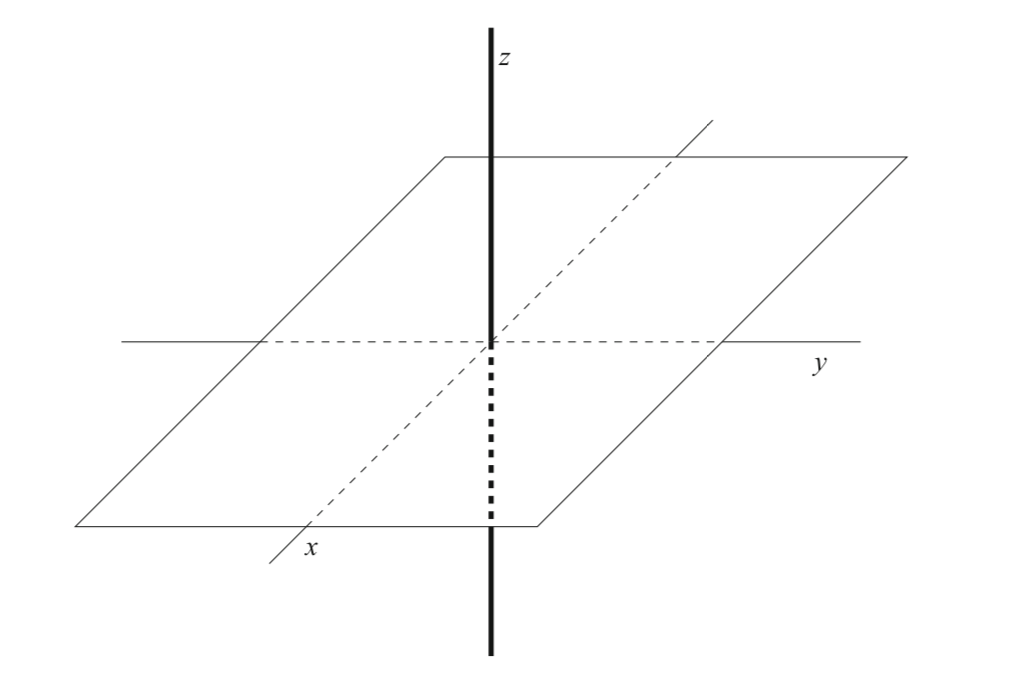
\includegraphics[width=1.0\textwidth]{affineVariety.png}
 	\caption[Example of an affine variety]{Affine variety defined by $(xz,yz)$. Image source: (\cite{algGeom}, page $9$).}
 	\label{fig1}
 \end{figure}

 \begin{DF}
Let $R$ be an commutative ring, then any non-empty subset $I \subseteq R$ is called a (two-sided) \textbf{ideal} of $R$ if it satisfies following requirements:
\begin{itemize}
\item $I \neq \emptyset,$\hfill ($I$ is a non-empty set)
\item $\forall f,g \in I: (f + g) \in I,$ \hfill ($I$ is closed under addition)
\item $\forall f \in I,\ \forall h \in R: hf \in I.$ \hfill ($I$ is closed under multiplication by $R$)
\end{itemize}
\end{DF}
\noindent In this thesis we are mostly concerned about ideals generated by a finite number of polynomials over some field.
\begin{DF}
Let $X = (x_1, \ldots ,x_n)$ be an ordered $n$-tuple of formal variables and let $f_1,\ldots,f_s \in \mathbb{F}[X] $ be an $s$-tuple of polynomials. Then we set
$$
\langle f_1, \ldots, f_x \rangle := \{ \sum_{i=1}^n h_if_i\ |\ h_1,\ldots,h_s \in \mathbb{F}[X]\}
$$
\end{DF}
\noindent to be the \textbf{ideal generated by} polynomials $f_1,\ldots,f_s$.
\begin{RM}
Every ideal $I$ of $\mathbb{F}[X]$ is finitely generated which means:
$$
\exists s \in \mathbb{N},\ \exists f_1,\ldots,f_s \in \mathbb{F}[X]: I = \langle f_1, \ldots, f_s \rangle,
$$
\noindent and we say that these polynomials $f_1,\ldots,f_s$ form a \textbf{basis} of $I$. Note that a given ideal $I$ may have many different bases. If we have two different bases $B_1 = (f_1,\ldots,f_s),\ s \in \mathbb{N},$ and $B_2 = (g_1, \ldots, g_t),\ t \in \mathbb{N},$ of the same ideal $I$ in $\mathbb{F}[X]$ such that $I = \langle B_1\rangle = \langle B_2 \rangle,$ then the affine varieties in $\mathbb{F}^n$ defined by the bases $B_1$ and $B_2$ are the same.
$$
\mathcal{V}(B_1) = \mathcal{V}(B_2).
$$
\end{RM}
\begin{DF}
Let $\mathcal{V} \subseteq \mathbb{F}^n$ be an affine variety and let $X = (x_1, \ldots ,x_n)$ be an ordered $n$-tuple of formal variables. Then we set 
$$
\mathbf{I}(\mathcal{V}) := \{ f \in \mathbb{F}[X]\ |\ \forall a \in \mathcal{V}: f(a) = 0\}.
$$
\noindent to be the \textbf{ideal of affine variety} $\mathcal{V}$.
\end{DF}
\begin{RM}
The natural question to ask is whether $\mathbf{I}(\mathcal{V}(f_1,\ldots,f_s)) = \langle f_1,\ldots,f_s \rangle.$ The answer, unfortunately, is not always yes, but the following set inclusion holds:
$$
\langle f_1,\ldots,f_s \rangle \subseteq \mathbf{I}(\mathcal{V}(f_1,\ldots,f_s)) .
$$
\end{RM} 
\subsection{Monomial Ordering}
\noindent The notion of ordering of terms in polynomial is a key ingredient in many algorithms, e.g. long division of polynomials. When dealing with polynomials in only one variable we usually write the terms of the polynomial in the decreasing order by their monomial degree. For example, $f(x) = 2x^4 - 10x^3 + x^2 + x -12$. The degree ordering on the one-variable monomials is straightforward:
$$
\cdots > x^{m+1} > x^m > x^{m-1} \cdots > x^2 > x > 1
$$
We would like to establish an ordering on the terms in polynomials in $\mathbb{F}[X],$ where $X = (x_1, \ldots, x_n)$. First, we note that we can reconstruct the monomial $X^{\alpha} = x_1^{\alpha_1}\cdots x_n^{\alpha_n}$ from the $n$-tuple of exponents $\alpha = (\alpha_1,\ldots, \alpha_n) \in \mathbb{Z}_{\geq 0}^n.$ Based on this observation we can define an ordering $>$ on the space $\mathbb{Z}_{\geq 0}^n$ which will also gives us an ordering on the monomials $\in \mathbb{F}[X].$ If for some $\alpha, \beta \in  \mathbb{Z}_{\geq 0}^n$ and some ordering $>$ holds: $\alpha > \beta$ we will also say that $X^\alpha > X^\beta.$ We will only consider \textbf{total orderings} which means that for every pair of monomials $X^\alpha$ and $X^\beta$, exactly one of the three statements holds:
\begin{itemize}
\item $X^\alpha > X^\beta,$\hfill (when $\alpha > \beta$)
\item $X^\alpha = X^\beta,$\hfill (when $\alpha = \beta$)
\item $X^\alpha < X^\beta,$\hfill (when $\alpha < \beta$)
\end{itemize}
\noindent and $>$ is transitive:
$$
\forall \alpha, \beta, \gamma \in \mathbb{Z}_{\geq 0}^n: (X^\alpha > X^\beta \land X^\beta > X^\gamma) \implies X^\alpha > X^\gamma.
$$
\noindent We also require that multiplication of two polynomials does not change the relative order of terms. Therefore the following property for $>$ must hold:
$$
\forall \alpha, \beta, \gamma \in \mathbb{Z}_{\geq 0}^n: X^\alpha > X^\beta \implies X^\alpha X^\gamma > X^\beta X^\gamma.
$$
\noindent Which in terms of the exponent vectors means: 
$$
\forall \alpha, \beta, \gamma \in \mathbb{Z}_{\geq 0}^n: \alpha > \beta \implies \alpha + \gamma > \beta + \gamma.
$$
\noindent To summarize all the requirements, we make the following definition.
\begin{DF}
A \textbf{monomial ordering} $>$ on $\mathbb{F}[X]$, where $X = (x_1, \ldots, x_n)$ is a relation $>$ on $\mathbb{Z}_{\geq 0}^n$ satisfying:
\begin{itemize}
\item $>$ is a total ordering on $\mathbb{Z}_{\geq 0}^n$,
\item $\forall \alpha, \beta, \gamma \in \mathbb{Z}_{\geq 0}^n: \alpha > \beta \implies \alpha + \gamma > \beta + \gamma,$
\item $\forall A \subseteq \mathbb{Z}_{\geq 0}^n,\ A \neq \emptyset: \exists \alpha \in A,\ \forall \beta \in A \setminus \{\alpha \}: \beta > \alpha.$ 
\end{itemize}
\noindent Last requirement tells us that in every non-empty subset of $\mathbb{Z}_{\geq 0}^n$ there exists a smallest element under the relation $>$.
\end{DF}
\phantom{.}
\phantom{.}
\noindent Now we will define a couple of standard monomial orderings.
\begin{DF}
Let $\alpha = (\alpha_1, \ldots, \alpha_n),\ \beta = (\beta_1, \ldots, \beta_n)\in \mathbb{Z}_{\geq 0}^n.$ \textbf{Lexicographic Order} (\textbf{lex}), denoted by $>_{lex}$, is a generalization of the way words are ordered in a dictionary. We say $\alpha >_{lex} \beta$ if the leftmost non-zero entry of the vector difference $\alpha - \beta \in \mathbb{Z}^n$ is positive. We will write: $X^\alpha >_{lex} X^\beta$ if $\alpha >_{lex} \beta$.
\end{DF}
For example:
\begin{itemize}
\item $(10,4,3) >_{lex} (10, 3, 4),$ since $\alpha - \beta = (0,1,-1)$.
\item $(7,5,3,1) >_{lex} (7, 5, 2, 4),$ since $\alpha - \beta = (0,0,1,-3)$.
\item The variables $x_1,\ldots,x_n$ are ordered in the usual way by the lexicographic order:
$$
(1,0,\ldots,0) >_{lex} (0,1,0,\ldots, 0) >_{lex} \cdots >_{lex} (0, \ldots, 0, 1),
$$
so $x_1 >_{lex} x_2 >_{lex} \cdots >_{lex} x_n.$ \\ \\
In the rest of the thesis we will also assume $x >_{lex} y >_{lex} z,$ unless stated otherwise.
\end{itemize} 
\begin{DF}
Let $\alpha = (\alpha_1, \ldots, \alpha_n),\ \beta = (\beta_1, \ldots, \beta_n)\in \mathbb{Z}_{\geq 0}^n.$ \textbf{Graded Lexicographic Order} (\textbf{grlex}), denoted by $>_{grlex}$, at first orders terms by the total degree, then break ties using the standard lexicographic order defined above. 
$$
\alpha >_{grlex} \beta: (|\alpha| > |\beta|) \lor (|\alpha| = |\beta| \land \alpha >_{lex} \beta),
$$
where $|\alpha| = \sum_{i=1}^n \alpha_i$ and $|\beta| = \sum_{i=1}^n \beta_i$.
\end{DF}
\begin{itemize}
\item $(10,2,6) >_{grlex} (10, 3,4),$ since $|\alpha| = 18 > |\beta| = 17$.
\item $(7,5,3,1) >_{grlex} (7, 5, 1, 3),$ since $|\alpha| = 16 = |\beta|$ and $\alpha >_{lex} \beta$.
\item The variables $x_1,\ldots,x_n$ are ordered the same way as by $>_{lex}$ order:
$$
(1,0,\ldots,0) >_{grlex} (0,1,0,\ldots, 0) >_{grlex} \cdots >_{grlex} (0, \ldots, 0, 1),
$$
\end{itemize} 
\begin{DF}
Let $\alpha = (\alpha_1, \ldots, \alpha_n),\ \beta = (\beta_1, \ldots, \beta_n)\in \mathbb{Z}_{\geq 0}^n.$ \textbf{Graded Reverse Lexicographic Order} (\textbf{grevlex}), denoted by $>_{grevlex}$, is somehow less intuitive order, but it is usually the most efficient for computations.  We say $\alpha >_{grevlex} \beta$ if $|\alpha| > |\beta|$ or if $|\alpha| = |\beta|$ and the rightmost non-zero entry of vector difference $\alpha - \beta \in \mathbb{Z}^n$ is negative.
\end{DF}
\begin{itemize}
\item $(4,7,1) >_{grevlex} (4, 2,5),$ since $|\alpha| = 12 > |\beta| = 11$.
\item $  (7, 5, 1, 3) >_{grevlex} (1,5,3,7),$ since $|\alpha| = 16 = |\beta|$ \\
\phantom{.}\hfill and $\alpha - \beta = (6,0,-2, -4),\ -4 < 0$.
\item The variables $x_1,\ldots,x_n$ are ordered the same way as by $>_{lex}$ order:
$$
(1,0,\ldots,0) >_{grevlex} (0,1,0,\ldots, 0) >_{grevlex} \cdots >_{grevlex} (0, \ldots, 0, 1),
$$
\end{itemize}
Now we will show how would the polynomial $f(x,y,z) = 4xy^2z + 4z^2 - 5x^3 + 7x^2z^2 \in \mathbb{Z}[x,y,z]$ be written if we reorder its terms by those standard monomial orderings.
\begin{itemize}
\item With respect to the lex order, we would reorder the terms of $f$ in decreasing order:
$$
f(x,y,z) = -5x^3 + 7x^2z^2 + 4xy^2z + 4z^2.
$$
\item With respect to grlex order:
$$
f(x,y,z) = 7x^2z^2  + 4xy^2z -5x^3 + 4z^2.
$$
\item With respect to grevlex order:
$$
f(x,y,z) = 4xy^2z + 7x^2z^2  -5x^3 + 4z^2.
$$
The first two terms have the same total degree of $4$ and $xy^2z >_{grevlex} x^2z^2$ because $(1,2,1) - (2,0,2) = (-1,2,-1)$ and $-1 < 0$.
\end{itemize} 
\begin{DF}
Let $f = \sum_\alpha a_\alpha X^\alpha$ be a non-zero polynomial in $\mathbb{F}[X]$ and let $>$ be a monomial order.
\begin{itemize}
\item The \textbf{multidegree} of $f$ is:
$$
\text{multideg}(f) := \text{max}(\alpha \in \mathbb{Z}_{\geq 0}^n\ |\ a_\alpha \neq 0),
$$
the maximum is taken with respect to $>$.\\ \\
Let $g \in \mathbb{F}[X],\ g \neq 0$, then multideg$(fg) = \text{multideg}(f) + \text{multideg}(g)$. If $(f + g) \neq 0$, then $\text{multideg}(f + g) \leq \text{max}(\text{multideg}(f),\ \text{multideg}(g))$, more precisely if the multidegrees of $f$ and $g$ are not equal, then the equality occurs: $\text{multideg}(f + g) = \text{max}(\text{multideg}(f),\ \text{multideg}(g))$.
\item The \textbf{leading coefficient} of $f$ is:
$$
\text{LC}(f) := a_{\text{multideg}(f)} \in \mathbb{F}.
$$
\item The \textbf{leading monomial} of $f$ is:
$$
\text{LM}(f) := X^{\text{multideg}(f)} \in \mathbb{F}[X],
$$
with coefficient $1$.
\item The \textbf{leading term} of $f$ is:
$$
\text{LT}(f) := (\text{LC}(f)\cdot \text{LM}(f)) \in \mathbb{F}[X].
$$
\end{itemize}
\end{DF}
\noindent To illustrate that, let $f(x,y,z) = 4xy^2z + 4z^2 - 5x^3 + 7x^2z^2 \in \mathbb{Z}[x,y,z]$ as before and lets use $>_{grevlex}$ order.
\begin{align*}
f(x,y,z) &= 4xy^2z + 7x^2z^2  -5x^3 + 4z^2, \text{ (in  grevlex order)}\\
\text{multideg}(f)&=(1,2,1), \\
\text{LC}(f)&=4, \\
\text{LM}(f)&=xy^2z, \\
\text{LT}(f)&=4xy^2z. \\
\end{align*}
Now we can formulate the idea of a general division algorithm in $\mathbb{F}[X]$.
\begin{RM}
Let $p, q \in \mathbb{F}[X]$ be two monomials, we say that the monomial $p$ is \textbf{divisible} by the monomial $q$ if and only if there exists a monomial $h \in \mathbb{F}[X]$ such that: $p = qh$. We denote it by $q\ |\ p$ which can be read  as \textbf{$\mathbf{q}$ divides $\mathbf{p}$}.
\end{RM}
\begin{DF}
Let $>$ be a monomial order on $\mathbb{Z}_{\geq 0}^n$, let $F = (f_1, \ldots, f_s)$ be an ordered $s$-tuple of polynomials in $\mathbb{F}[X],$ where $X = (x_1, \ldots, x_n)$. Then every $f \in \mathbb{F}[X]$ can be written as:
$$
f = q_1f_1 + \cdots + q_sf_s + r,
$$
where $q_i, r \in \mathbb{F}[X]$, and either $r = 0$ (is a zero polynomial) or $r$ is a linear combination, with coefficients in $\mathbb{F}$, of monomials $\in \mathbb{F}[X]$, none of those monomials is divisible by any of LT$(f_1), \ldots,$LT($f_s$).
We call polynomial $r$ a \textbf{remainder} of $f$ on division by $F$. Furthermore, if $q_if_i \neq 0$, then
$$
\text{multideg}(f) \geq \text{multideg}(q_if_i).
$$
\end{DF}
\noindent The algorithm itself will be presented in the chapter \ref{Algorithms}. Unfortunately,  the remainder is not uniquely characterized and depends on the order of the divisors in the set $F$ and also on the monomial order itself. \\ \\
\noindent Furthermore, we would like to use this idea to answer the ideal membership problem. Let $f, f_1, \ldots, f_s \in \mathbb{F}[X]$ and let $I = \langle f_1, \ldots, f_s \rangle$ be an ideal. We would like to determine whether $f \in I$ is true. We can clearly state that if the remainder $r$ obtained after division of $f$ by $F = (f_1, \ldots, f_s)$ is $0$, then $f$ has to be an element of the ideal $I$. So $r=0$ is a sufficient condition for the ideal membership, however it isn't a necessary condition for $f$ being in the ideal. To remedy this situation we will try to describe a "good" basis of the ideal $I$, such that the remainder $r$ on division by the polynomials of this basis will be uniquely determined and that the condition $r=0$ will be equivalent to the membership in the ideal. Exactly those good properties have Gröbner bases which we are gonna describe in the following section.
\section{Gröbner Bases}
\begin{DF}
An ideal $I \subseteq \mathbb{F}[X]$ is called a \textbf{monomial ideal} if there exists a (possibly infinite) subset $A \subseteq \mathbb{Z}_{\geq 0}^n$ such that $I$ consists of all polynomials which are finite sums: $\sum_{\alpha \in A} h_\alpha X^\alpha$, where $h_\alpha \in \mathbb{F}[X].$ We can then write $I$ in the form: $I = \langle X^\alpha \ |\ \alpha \in A\rangle.$ Monomial $X^\beta, \beta \in \mathbb{Z}_{\geq 0}^n,$ lies in ideal $I$ if and only if there exist $\alpha \in A$, such that $X^\alpha \ |\ X^\beta$ ($X^\beta$ is divisible by some $X^\alpha$). 
\end{DF}
\begin{RM}
\textbf{(Dickson's Lemma).} Any monomial ideal $I = \langle X^\alpha \ |\ \alpha \in A\rangle \subseteq \mathbb{F}[X]$ can be written in the form $I = \langle X^{\alpha(1)}, \ldots, X^{\alpha(s)}\rangle,\ s \in \mathbb{N},$ where $\alpha(1), \ldots, \alpha(s) \in A$. In particular, $I$ has a finite basis $(X^{\alpha(1)}, \ldots, X^{\alpha(s)})$.
\end{RM}
\begin{DF}
A monomial ideal $I \subseteq \mathbb{F}[X]$ has a finite basis $(X^{\alpha(1)}, \ldots, X^{\alpha(s)})$ with the property that $X^{\alpha(i)}$ does not divide $X^{\alpha(j)}$ for any $i \neq j$. Furthermore, this basis is unique and is called the \textbf{minimal basis} of $I$.
\end{DF}
\begin{DF}
Let $I \subseteq \mathbb{F}[X],\ I \neq {0},$ be an ideal and fix a monomial ordering on $\mathbb{F}[X]$.  Then:
\begin{itemize}
\item We denote by LT$(I)$ the \textbf{set of leading terms} of non-zero elements of~$I$.
$$
\text{LT}(I) = \{ cX^\alpha \ |\ \exists f \in I \setminus \{0\}: \text{LT}(f)= cX^\alpha \}.
$$
\item We denote by $\langle \text{LT}(I) \rangle$ the \textbf{ideal of leading terms} of $I$. $\langle \text{LT}(I) \rangle$ is a monomial ideal, therefore there exist a finite set $g_1,\ldots, g_t \in I,\ t \in \mathbb{N},$ such that:
$$
\langle \text{LT}(I) \rangle = \langle \text{LT}(g_1), \ldots, \text{LT}(g_t) \rangle.
$$
\end{itemize}
\end{DF}
\begin{DF}
Fix a monomial order on $\mathbb{F}[X]$, therefore every polynomial $f \in \mathbb{F}[X]$ has an unique leading term. A finite subset $G = \{g_1, \ldots, g_t \}$ of an ideal $I \subseteq \mathbb{F}[X],\ I \neq \{ 0 \}$ is said to be a \textbf{Gröbner basis} (or \textbf{standard basis}) if:
$$
\langle \text{LT}(g_1), \ldots, \text{LT}(g_t) \rangle = \langle \text{LT}(I) \rangle.
$$
Additionally we define the Gröbner basis of the zero ideal $\{0\}$ to be the empty set $\emptyset$ using the convention that $\langle \emptyset \rangle = \{0\}.$
\end{DF}
\begin{RM}
Every ideal $I \subseteq \mathbb{F}[X]$ has a Gröbner basis. Furthermore, any Gröbner basis for an ideal $I$ is a basis of $I$. The theory of Gröbner bases was developed by B. Buchberger in his PhD thesis (1965) and named after his thesis's advisor W. Gröbner. Buchberger also developed fundamental algorithms to find and work with Gröbner bases. In many computer algebra systems there is usually used an alternative spelling "Groebner bases".
\end{RM}
\phantom{.}
\phantom{.}
\noindent Now we will mention few important properties of Gröbner bases.
\begin{RM}
Let $I \subseteq \mathbb{F}[X]$ be an ideal and let $G = \{g_1, \ldots, g_t\}$ be a Gröbner basis of $I$. Then for any $f \mathbb{F}[X],$ there is an unique polynomial $r$ with those two properties:
\begin{itemize}
\item No term of $r$ is divisible by any of LT$(g_1),\ldots,$LT$(g_t)$.
\item $\exists g \in I:\ f = g + r.$
In particular, $r$ is the remainder on division of $f$ by set $G$ no matter how are the elements of $G$ listed when using the division algorithm. 
\end{itemize}
Polynomial $r$ is called the \textbf{normal form} of f. \\ \\ 
\noindent Polynomial $f \in I$ if and only if the remainder $r$ on division $f$ by $G$ is zero, $r = 0.$
\end{RM}
\begin{DF}
Let $f \in \mathbb{T}[X]$ be an polynomial and let $F = (f_1, \ldots, f_s) \subseteq \mathbb{T}[X]$ be an ordered $s$-tuple of polynomials. We will denote the remainder on the division of $f$ by $F$ by $\overline{f}^F$. If $F$ is a Gröbner basis for $\langle f_1, \ldots, f_s \rangle$, then we can regard $F$ as a set without any particular order, because the remainder on the division by a Gröbner basis is unique.
\end{DF}

%properties of GBases
%BCHberg criterium
%
%Define VectorSpace?
%Divison Res => alg in the next section with F4, F5
%
%Schoof–Elkies–Atkin algorithm - pocet bodu na EC 
\chapter{Elliptic Curves and Discrete Logarithm Problem}
\section{Elliptic Curves}
This section's main focus will be elliptic curves and groups of points on those elliptic curves. At first we are going to define what is a general elliptic curve, after that we will define an operation on the set of points on elliptic curve that with "the point in infinity" form an Abelian group. This section is based mostly on \cite{mky}.
\begin{DF}
An \textbf{elliptic curve} over a (prime order) finite field $GF(p),$ \\ $p > 3,\ p$ prime, defined by the short Weierstrass equation, is a set:
$$
E(GF(p)) := \{(x,y)\ |\ x,y \in \mathbb{T},\ y^2 = x^3 + Ax+B\} \cup \{ \mathcal{O} \},
$$
where $A, B \in GF(p)$ are \textbf{coefficients of the elliptic curve} and the \textbf{discriminant} of the elliptic curve, denoted by $\Delta$, is non-zero. Point $\mathcal{O}$ is called the \textbf{point at infinity} (in the projective plane).
\begin{align*}
\Delta = -16(4A^3 + 27B^2) \neq 0.
\end{align*}
Curves satisfying this condition are called \textbf{non-singular} and the right-hand-side polynomial ($x^3 + Ax+B$) in $x$ has 3 distinct roots. 
\end{DF}
\begin{DF}
Let $E(GF(p))$ be an elliptic curve and let $P,Q \in E(GF(p)),\ P=(x_1,y_1),\ Q=(x_2,y_2)$ be two points on the elliptic curve $E$. We define the binary operation $\oplus: E(GF(p)) \times E(GF(p)) \to E(GF(p))$, called \textbf{addition on the elliptic curve} $E(GF(p))$, as follows:
\begin{itemize}
\item Point at infinity $\mathcal{O}$ is an identity element of the operation $\oplus$, therefore if $P = \mathcal{O},\ P \oplus Q = Q,$ or if $Q = \mathcal{O},\ P \oplus Q = P.$
\item Else if $x_1 = x_2$ and $P\neq Q$, $P\oplus Q = \mathcal{O}.$ Point at infinity $\mathcal{O}$ is the identity element of the operation $\oplus$, therefore point $Q$ is the \textbf{additive inverse} of the point $P$, denoted by $\ominus P$. We can now state the explicit formula for the point $\ominus P$, we know its $x$-coordinate is $x_1$, and we will use the $E$ equation and substitute $X$ with $x_1$:
$$
Y^2  = (x_1^3 + Ax_1 + B),
$$
which is a quadratic equation in the variable $Y$ and we already know one of its roots, which is $y_1$, the other root has to be $-y_1$, therefore point $\ominus P = (x_1, -y_1).$
\item Else if $x_1 \neq x_2$, let $\lambda$ be the slope of the line defined by the points $P,Q.$
$$
\lambda = \frac{y_2 - y_1}{x_2 - x_1},
$$
else if $P = Q$ (\textbf{point doubling}), let $\lambda$ be the slope of the tangent line to the elliptic curve equation at the point $P.$
$$
\lambda = \mathlarger{\mathlarger{\frac{\frac{\mathrm{d}E}{\mathrm{d}X}}{\frac{\mathrm{d}E}{\mathrm{d}Y}}}}(x_1, y_1) = \frac{3x_1^2+ A}{2y_1}, 
$$
where $\frac{\mathrm{d}E}{\mathrm{d}X}, \frac{\mathrm{d}E}{\mathrm{d}Y}$ is the derivative of the elliptic curve equation with respect to $X,Y$. \\
The result of the operation $\oplus$ is:
\begin{align*}
x_3 &= \lambda^2 - x_1 - x_2, \\
y_3 &= \lambda(x_1 - x_3) - y_1, \\ 
 P \oplus Q &= (x_3, y_3).
\end{align*}
\end{itemize}
\end{DF}
\begin{DF}
A set of points on the elliptic curve defined by the short Weierstrass equation and the binary operation $\oplus$ form an Abelian group, $(E(GF(p)), \oplus)$ is a group and we denote it by $E$, or if we want to explicitly mention the coefficients $A,B$ and the prime field $GF(p),$ we use $E(A,B,p)$.
\end{DF}
\begin{NRM}
Let $P \in E$ be a point on an elliptic curve $E$ with group operation $\oplus$. To shorten the notation of the repeated application of the group law we will use the notation introduced in chapter 1. To remind our readers: \textbf{multiplication} of a point on the elliptic curve $E$ by an integer has the following meaning:
$$
\forall P \in E,\ \forall t \in \mathbb{Z}: tP := \begin{cases} \underbrace{P \oplus P \oplus \cdots \oplus P}_{\text{t-times}} &\quad t > 0, \\
\mathcal{O} \text{ (identity element) } &\quad t = 0, \\
\underbrace{(\ominus P) \oplus (\ominus P) \oplus \cdots \oplus (\ominus P)}_{\text{t-times}} &\quad t < 0.
\end{cases}
$$
\end{NRM} 
\begin{RM}
The complexity of arithmetic operations on $E$ is based on the complexity of operations in the underlying finite field $GF(p)$.  Exact number of arithmetic operations depends on the used algorithm and on the architecture of the CPU where it's executed. Table \ref{tblComp} provides a brief summary of the relationship between the operations on elliptic curve $E$ and number of arithmetic operations in the underlying finite field $GF(p)$. Addition in $GF(p)$ is denoted by $a_p$, multiplication in $GF(p)$ is denoted by $\cdot_p$, last column is the number of multiplicative inverses in $GF(p)^{\times}$. 
\begin{table}[!h]
\centering
\begin{tabular}{ |c||c|c|c| } 
 \hline
 & \# $+_p$ & \# $\cdot_p$ & \# mult. inverses \\ 
 \hline
 \hline
$\ominus P$ & 1 & 0 & 0  \\  \hline
$P \oplus Q, P \neq Q$ & 6 & 3 & 1 \\  \hline
$P \oplus Q, P = Q$ & 5 & 5 & 1 \\  \hline
$tP,\ t \in \mathbb{Z}_{\geq 0},\ k = \mathlarger{\lceil} \log_2(t) \mathlarger{\rceil}$ & $ (5k + 0.5k)$\footnotemark & $5k$ & 0 \\ \hline
\end{tabular}
\caption{Complexity of the arithmetic operations on the elliptic curve $E$ over $GF(p)$.}
\label{tblComp}
\end{table}
\end{RM}
\noindent We denote the number of bits of $p$ by $n = \mathlarger{\lceil} \log_2(p) \mathlarger{\rceil}$, then addition in $GF(p)^{+}$ is asymptotically $O(n)$, multiplication in $GF(p)^{\times}$, using Montgomery method \cite{handbook}, is $O(n^2)$ and multiplicative inverse in $GF(p)^{\times}$, using a careful implementation of the extended Euclidean algorithm (EEA) \cite{handbook}, is $O(n^2)$. An alternative to the EEA for calculating a multiplicative inverse in $GF(p)^{\times}$ is based on the Lagrange's theorem \ref{lagrange}. 
\begin{align*}
\forall a \in GF(p)^{\times},\ \exists n \in \mathbb{N}: \#a \cdot n = \#GF(p)^{\times} &= p - 1, \\ 
\forall a \in GF(p)^{\times}: a^{\#a} = 1 \implies a^{\#a - 1} &= a^{-1}, \\
\forall a \in GF(p)^{\times}: a^{-1} &= a^{p-2}.
\end{align*}
To calculate $a^{p-2}$ we can use the standard algorithm called square-and-multiply, for details see \cite{mky}, which has the same complexity $O(n^2)$ as the EEA.
\footnotetext{Using signed binary expansion of $t$ for the double-and-add algorithm, see \cite{mky} page 105.}
\begin{DF}

\end{DF}
\section{Discrete Logarithm Problem}
Let $y = b^x$, given $y \in \mathbb{R}_{> 0}$ and the base $b \in \mathbb{R}_{>0}$, we are asked to find the exponent $x \in \mathbb{R}$. We can rewrite this problem from the exponential form to the logarithmic form: $x = \log_b(y)$, to find the $x$ we can easily evaluate it on a calculator (using change of logarithm basis rule). Even if we didn't know the inverse function (logarithm), the exponential function is a strictly increasing function, therefore we could have just guessed a random $x_0$, evaluate $b^{x_0}$, compare it with $y$ and we would immediately know whether the solution $x$ is bigger/equal/lesser than $x_0$.
\\
\\
\noindent If we were given the same problem in a finite group, instead of over the real numbers, the situation would be significantly more complicated.
\begin{DF}
Let $G = (M, \cdot)$ be a group and let $h = g^x$, given $h \in M$ and the base $g \in M,\ \langle g \rangle = G,$ we are asked to find the exponent $x$~$\in$~$\{1, 2, \ldots, \#G\}.$ We call $x$ the \textbf{discrete logarithm} of $h$ with respect to the base $g$ and denote it by $x= \log_g(h)$. Problem of finding the solution $x$ is therefore called the \textbf{discrete logarithm problem} (DLP). We have decided to demand $g$ to be a generator of $G$ in order to guarantee the existence of the solution to the DLP.  
\end{DF}
\noindent To illustrate the difficulty of solving the DLP. Lets consider the multiplicative group $G$ of the finite field $GF(19).$ $G = (\{1,2,\ldots,18\}, \cdot_{19})$ and its generator $g=3,\ g \in G$. Group structure is shown on the figure \ref{fig2}. We might be asked to find such $k$, that $3^k \equiv 4 \text{ (mod 19)}$. 
 \begin{figure}[h]
\hspace*{-2cm}
 	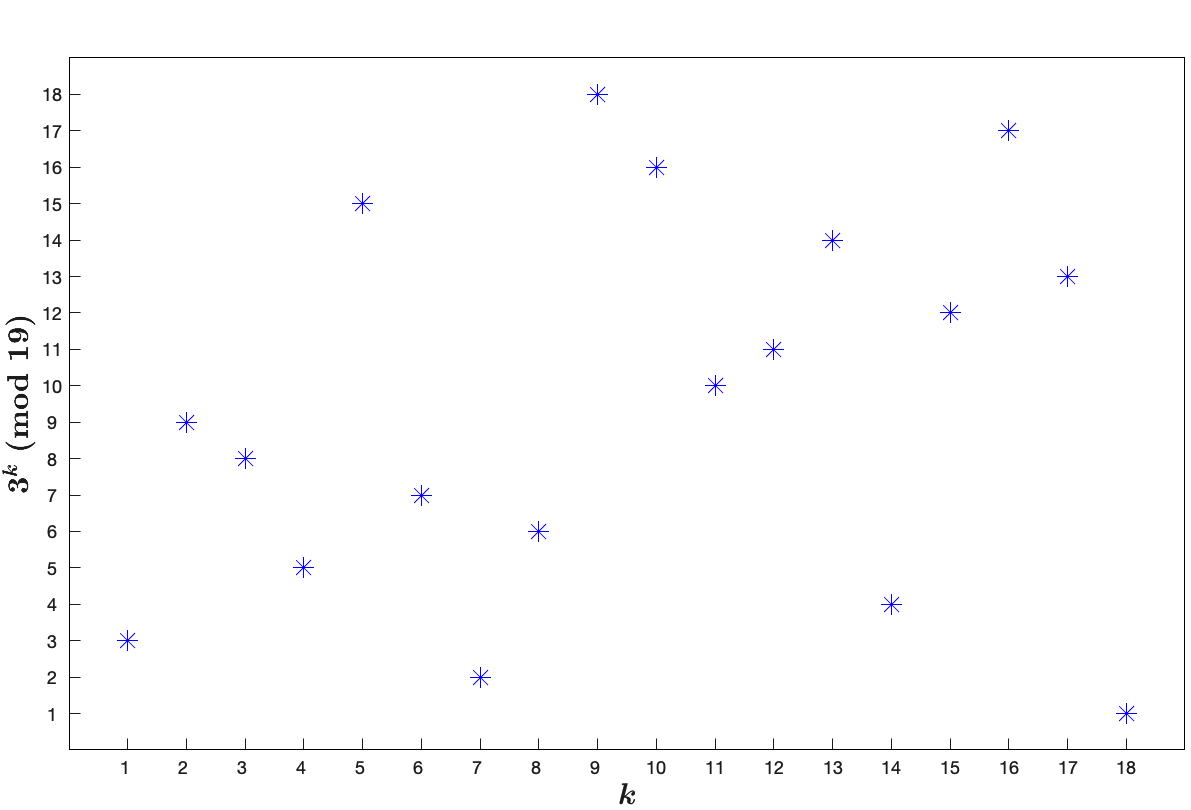
\includegraphics[width=1.25\textwidth]{graph3in19.png}
 	\caption[Example of the group structure of $GF(19)^\times$.]{Powers of the generator $g = 3$ in $GF(19)^\times$. Image was created by the author himself.}
 	\label{fig2}
 \end{figure}
 \newpage
\noindent Unfortunately, the function $g^k \text{ (mod 19)},\ k \in \mathbb{N},$ isn't monotonic, therefore we can't use the idea of trying a randomly selected $k_0$ and comparing $3^{k_0} \text{ (mod 19)}$ with $4$, but we can use the fact that the group $G$ is finite and its order is $\#G = 18 \implies 3^{18} \equiv 1 \text{ (mod 19)}.$ We can just try all possible values of $k \in \{0, 1, \ldots, 17\}$ and find the answer. This method is called the \textbf{brute-force attack}. 
\begin{align*}
3^0 \equiv 1 \text{ (mod 19)} &\not\equiv 4 \text{ (mod 19)}, \\
3^1 \equiv 3 \text{ (mod 19)} &\not\equiv 4 \text{ (mod 19)}, \\
3^2 \equiv 9 \text{ (mod 19)} &\not\equiv 4 \text{ (mod 19)}, \\
3^3 \equiv 8 \text{ (mod 19)} &\not\equiv 4 \text{ (mod 19)}, \\
&\vdots \quad \vdots \\
3^{13} \equiv 14 \text{ (mod 19)} &\not\equiv 4 \text{ (mod 19)}, \\
3^{14} &\equiv 4 \text{ (mod 19)}.
\end{align*}
The solution of this DLP is therefore $k = 14$ and we can see that the brute-force approach is very lengthy even for DLP in groups of small order. Complexity of solving the DLP in a group $G$ using the brute-force attack is $O(\#G)$ of group operations.
\begin{RM}
Standard properties of the logarithm may be used in the discrete logarithm case as well. Let $G$ be a finite Abelian group and let $g$ be a generator of $G$.
\begin{itemize}
\item $\forall p, q \in G: \log_g(pq) \equiv log_g(p) + log_g(q) \text{ (mod $\#G$)}$,
\item $\forall p, q \in G: \log_g(p(q)^{-1}) \equiv log_g(p) - log_g(q) \text{ (mod $\#G$)}$,
\item $\forall k \in \mathbb{Z},\ p \in G: \log_g(p^k) \equiv k \cdot log_g(p) \text{ (mod $\#G$)}$,
\item $h \in G,\ \langle h \rangle = G,\ \forall p \in G: log_g(p) \equiv log_h(p) \cdot log_g(h)  \text{ (mod $\#G$)}$.
\end{itemize}
Last property is the well-known change-of-base formula and tells us that if we are able to effectively solve the DLP with respect to some base we can use it to effectively solve the DLP with respect to any other base.
\end{RM}
\section{ECDLP description}
\section{General algorithms solving ECDLP}
\section{Summation Polynomials}
\chapter{Realisation in SageMath}

\chapter{Experimental Results}
poly division alg
Pohling-Hellmann
Pollard-Rho
BsGs
Groebner basic
F4, F5 Groebner
SumPoly 

\setsecnumdepth{part}
\chapter{Conclusion}


%\bibliographystyle{iso690}
%\bibliography{bibliography}
\begin{thebibliography}{10}

%\bibitem{Abel} THE EDITORS OF ENCYCLOPAEDIA BRITANNICA. \textit{Niels Henrik Abel: NORWEGIAN MATHEMATICIAN.} Encyclopaedia Britannica [online]. Apr 2, 2019 [Accessed on 2019-04-10]. Available at: \url{https://www.britannica.com/biography/Niels-Henrik-Abel}

\bibitem{algGeom} {COX, David A., John LITTLE and Donal O'SHEA. \textit{Ideals, Varieties, and Algorithms: An Introduction to Computational Algebraic Geometry and Commutative Algebra.} Fourth Edition. New York: Springer, 2015. Undergraduate texts in mathematics. ISBN 978-3-319-16721-3.}

\bibitem{mky} {KALVODA, Tomáš, Ivo PETR and Štěpán STAROSTA. Matematika pro kryptologii [online]. KAM FIT ČVUT. [Praha], Updated on 20-02-2019 [Accessed on 16-04-2019]. Available at: \url{https://courses.fit.cvut.cz/MI-MKY/media/lectures/mi-mky-poznamky-v17.pdf}}

\bibitem{myBP} {HOLLMANN, Matyáš. \textit{Implementace násobení na neasociativních (nekomutativních) algebrách.} Praha, 2017. Bakalářská práce. České vysoké učení technické v Praze, Fakulta informačních technologií. Vedoucí práce Jiřina Scholtzová. Available at: \url{https://dspace.cvut.cz/bitstream/handle/10467/69263/F8-BP-2017-Hollmann-Matyas-thesis.pdf}}

\bibitem{coset}{BRAY, Nicolas. \textit{Coset}. From MathWorld-A Wolfram Web Resource [online], created by Eric W. Weisstein. [Accessed on 16-04-2019]. Available at : \url{http://mathworld.wolfram.com/Coset.html}}

\bibitem{handbook}{COHEN, Henri, Gerhard FREY and Roberto AVANZI. \textit{Handbook of elliptic and hyperelliptic curve cryptography.} Boca Raton: Taylor and Francis, 2006. ISBN 978-1-58488-518-4.}


\end{thebibliography}
%citace

\setsecnumdepth{all}
\appendix

\chapter{Acronyms}
% \printglossaries
\begin{description}
	\item[EEA] Extended Euclidean algorithm
	\item[DLP] Discrete logarithm problem
	\item[ECDLP] Elliptic curve discrete logarithm problem
\end{description}


\chapter{Contents of enclosed CD}

%change appropriately

\begin{figure}
	\dirtree{%
		.1 readme.txt\DTcomment{the file with CD contents description}.
		.1 exe\DTcomment{the directory with executables}.
		.1 src\DTcomment{the directory of source codes}.
		.2 wbdcm\DTcomment{implementation sources}.
		.2 thesis\DTcomment{the directory of \LaTeX{} source codes of the thesis}.
		.1 text\DTcomment{the thesis text directory}.
		.2 thesis.pdf\DTcomment{the thesis text in PDF format}.
		.2 thesis.ps\DTcomment{the thesis text in PS format}.
	}
\end{figure}

\end{document}
